% Opener for December 2, 2026: Pat's mail route (five-house visiting-order puzzle)
% Build in a scratch directory: pdflatex mail-route.tex, then copy to ../2026-12-02-opener.pdf
% Every puzzle here is checked for exactly one answer by mail-route_check.py.
% The five-house town is the Week 10 house town (packet page 1) and the floor town:
% green A top, purple B upper left, yellow C upper right, blue D bottom left, red E bottom right.
\documentclass[11pt]{article}
\usepackage[letterpaper,margin=0.5in]{geometry}
\usepackage[T1]{fontenc}
\usepackage[default]{sourcesanspro}
\usepackage{tikz}
\usetikzlibrary{calc}
\usepackage{ragged2e}
\pagestyle{empty}
\setlength{\parindent}{0pt}
\definecolor{cgreen}{HTML}{3BA55C}\definecolor{cblue}{HTML}{3B73D6}
\definecolor{cred}{HTML}{D83A3A}\definecolor{cyellow}{HTML}{F2C318}
\definecolor{cpurple}{HTML}{7E4BB0}
% \house{name}{x,y}{colour}{word}: a coloured house with a white box for the visit number
\newcommand{\house}[4]{%
  \coordinate (#1) at (#2);
  \fill[#3!35!white,draw=#3!80!black,line width=1pt]
    ($(#2)+(-0.75,-0.65)$) -- ++(1.5,0) -- ++(0,0.95) -- ++(-0.75,0.6) -- ++(-0.75,-0.6) -- cycle;
  \draw[fill=white,line width=0.6pt] ($(#2)+(-0.36,-0.55)$) rectangle ++(0.72,0.72);
  \node[font=\small\bfseries,below,fill=white,inner sep=1pt] at ($(#2)+(0,-0.66)$) {#4};}
\newcommand{\road}[2]{\draw[line width=9pt,gray!30,line cap=round] (#1) -- (#2);}
\newcommand{\fivetown}{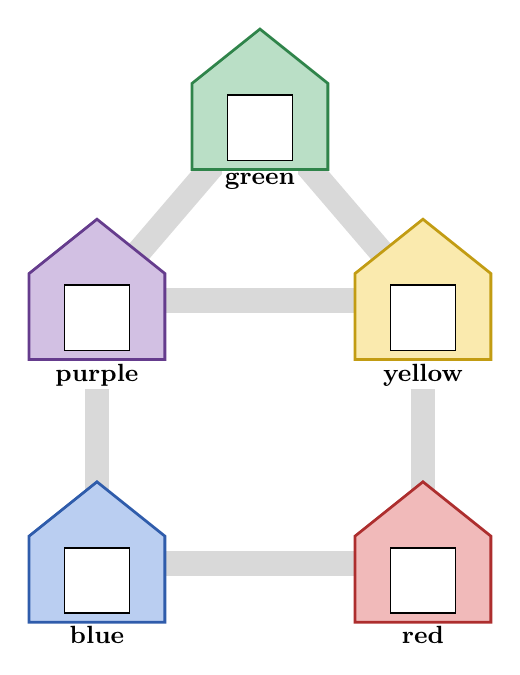
\begin{tikzpicture}[scale=1.15]
  \path (0,0) coordinate (D) (3.6,0) coordinate (E) (0,2.9) coordinate (B) (3.6,2.9) coordinate (C) (1.8,5.0) coordinate (A);
  \road{A}{B}\road{A}{C}\road{B}{C}\road{B}{D}\road{C}{E}\road{D}{E}
  \house{A}{1.8,5.0}{cgreen}{green}\house{B}{0,2.9}{cpurple}{purple}\house{C}{3.6,2.9}{cyellow}{yellow}
  \house{D}{0,0}{cblue}{blue}\house{E}{3.6,0}{cred}{red}
  \end{tikzpicture}}
\newenvironment{half}{\begin{minipage}[t][0.475\textheight][t]{\linewidth}\large\RaggedRight}{\end{minipage}}
\newcommand{\cutline}{\par\noindent\begin{tikzpicture}\draw[dashed,gray] (0,0)--(\linewidth,0);\end{tikzpicture}\par\vspace{0.3in}}
\newcommand{\heading}[1]{{\LARGE\bfseries #1}\hfill {\normalsize Name:} \rule{1.8in}{0.4pt}\par\medskip}
% \twocol{text}{picture}
\newcommand{\twocol}[2]{\begin{minipage}[t]{0.56\linewidth}\vspace{0pt}#1\end{minipage}\hfill
  \begin{minipage}[t]{0.40\linewidth}\vspace{0pt}\centering #2\end{minipage}}
\newcommand{\mainpuzzle}{%
  \heading{Pat's mail route}
  Pat the mail carrier brought one letter to each of these five houses, one house after another.
  Write 1 in the house Pat went to first, 2 in the next one, and so on up to 5.\par
  \medskip
  \twocol{%
  \begin{enumerate}\setlength{\itemsep}{6pt}
  \item Pat went to the red house right after the blue house.
  \item Pat went to the green house right after the yellow house.
  \item Pat went to the yellow house some time after the red house.
  \item The green house was not the last house.
  \end{enumerate}\par
  \medskip
  \textbf{Done?} Cross out clue 4. Find every order that fits now. Write a new clue that makes it exactly one again.}{\fivetown}}
\begin{document}
\begin{half}\mainpuzzle\end{half}
\cutline
\begin{half}\mainpuzzle\end{half}
\newpage
\begin{half}
\heading{Pat's mail route (three houses)}
Pat brought one letter to each of these three houses, one house after another.
Write 1 in the house Pat went to first, then 2, then 3.\par
\medskip
\twocol{%
\begin{enumerate}\setlength{\itemsep}{6pt}
\item Pat went to the yellow house right after the purple house.
\item Pat did not start at the green house.
\end{enumerate}\par
\medskip
\textbf{Done?} Try the five-house puzzle.}{%
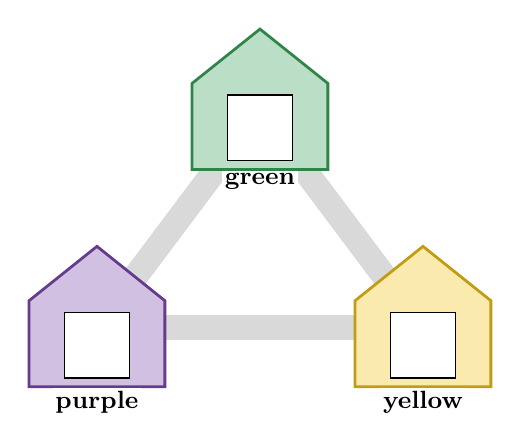
\begin{tikzpicture}[scale=1.15]
  \path (0,0) coordinate (B) (3.6,0) coordinate (C) (1.8,2.4) coordinate (A);
  \road{A}{B}\road{A}{C}\road{B}{C}
  \house{A}{1.8,2.4}{cgreen}{green}\house{B}{0,0}{cpurple}{purple}\house{C}{3.6,0}{cyellow}{yellow}
\end{tikzpicture}}
\end{half}
\cutline
\begin{half}
\heading{Pat's mail route (follow the paths)}
Pat brought one letter to each of these five houses, one house after another. From each house,
Pat walked along one path straight to the next house. Write 1 in the house Pat went to first,
and so on up to 5.\par
\medskip
\twocol{%
\begin{enumerate}\setlength{\itemsep}{6pt}
\item Pat started at a bottom house.
\item Pat went to the red house right after the blue house.
\item The top house was not first and not last.
\end{enumerate}\par
\medskip
\textbf{Done?} Write your own route puzzle with exactly one answer, and give it to a friend.}{\fivetown}
\end{half}
\end{document}
